\documentclass{article}%
\usepackage[T1]{fontenc}%
\usepackage[utf8]{inputenc}%
\usepackage{lmodern}%
\usepackage{textcomp}%
\usepackage{lastpage}%
\usepackage{authblk}%
\usepackage{graphicx}%
%
\title{Functional CD40 Expression Induced following Bacterial Infection of Mouse and Human Osteoblast}%
\author{Karen Hunter}%
\affil{Second Department of Internal Medicine, Tottori University School of Medicine, Tottori 683{-}8504, Japan}%
\date{01{-}01{-}2009}%
%
\begin{document}%
\normalsize%
\maketitle%
\section{Abstract}%
\label{sec:Abstract}%
In one of the first clinical trials to directly convert stem cells to myocytes, researchers at Monash University, in Australia, discovered that it triggered powerful but undetectable cellular transcription factors, which work together to enhance differentiation.\newline%
MyoD, a pro{-}inflammatory cytokine, was released during the MYOLESTOM muscle stem cell propagation trial. However, study participants were unable to fully activate their microglia  the proteins responsible for controlling behavior in the body. IcyT cells were less eager to produce myoD due to previously undetectable cellular transcription factors boosting the cytokine.\newline%
The study team conducted this study to discover how genes produced during myocyte development can also affect gene expression. Our new findings suggest that myocrit proteins may provide a window into a biological process that can turn genes on or off  in other words, you can turn genes on and off  in a very unexpected way, said lead investigator of the study, Professor Barbara Olehers, from Monashs Institute of Biomedical Informatics.\newline%
A key objective of this research is to develop the appropriate therapy to improve the fitness of the muscle muscles. MyoD therapeutics are currently being tested in other clinical trials and this research has the potential to show how myocrit proteins cause physiological changes not seen in animal models. Our findings suggest that MYOCR{-}MyoD might also be a potential therapeutic agent against myovidrosis, a rare muscle disorder, says Olehers.\newline%
Professor Paul Nielse, Director of the Clinical Research Center, Sydney and Professor of Genetics at the Gosthenes Institute at Monash, explains that myocrit proteins suppress myoD in over 70 per cent of people with myovidrosis. Myocrit{-}MyoD is the main cellular transcription factor in myosin 1, myosin 2, TCR1 and TCR22, and acts as a master regulator in the cell. It influences protein synthesis and the function of all myosin genes. It also interacts with neurons and organ tissues directly, via multiple channels.\newline%
Our findings will help us understand the mechanisms that contribute to myosin{-}mediated myosin production in myowoserydzolysis, adds Nielse.\newline%
The study was supported by the National Health and Medical Research Council (1K021376) and the Australian Institute of Cancer Research (1K010739). The Monash University Institute of Biomedical Informatics has also received funding from the Garman Foundation and the Australian Cancer Foundation.

%
\subsection{Image Analysis}%
\label{subsec:ImageAnalysis}%


\begin{figure}[h!]%
\centering%
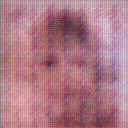
\includegraphics[width=150px]{500_fake_images/samples_5_44.png}%
\caption{A Black And White Photo Of A Black And White Cat}%
\end{figure}

%
\end{document}